\documentclass[aps,prl,reprint,amsmath,amssymb,nofootinbib,raggedbottom]{revtex4-2}
\usepackage[T1]{fontenc}
\usepackage{bm}
\usepackage{tikz}
\usetikzlibrary{arrows.meta}
\definecolor{mpoblue}{HTML}{5B9DBD}
\definecolor{mpored}{HTML}{D9666B}
\tikzset{
 tensor/.style={draw=black,fill=mpoblue,line width=.6pt,
   minimum width=.18cm,minimum height=.18cm,inner sep=0pt},
 wire/.style={draw=black,line width=.6pt},
 arrow/.style={-{Latex[length=1.5mm]},line width=.6pt}
}
\usepackage[colorlinks=true,citecolor=blue,linkcolor=blue,urlcolor=blue]{hyperref}
\hypersetup{pdftitle={A short diagrammatic explanation of the spin-1 Haldane gap proof}}
\newcommand{\Tr}{\operatorname{Tr}}
\newcommand{\Ps}{P_{\mathrm{s}}}
\newcommand{\Pt}{P_{\tau}}
\newcommand{\trv}{\operatorname{Tr}_{\mathrm v}}
\newenvironment{proofdiagram}{\par\smallskip\noindent\begin{minipage}{\columnwidth}\centering}{\end{minipage}\par\smallskip}
% A closed spacetime patch. Its opposite boundaries are identified.
% Arguments: lower-left x, lower-left y, number of columns, number of rows.
\newcommand{\netpatch}[4]{%
 \begin{scope}[shift={(#1,#2)}]
 \fill[mpoblue!10] (0,0) rectangle ({.4*#3},{.4*#4});
 \draw[black!35,densely dashed,line width=.35pt]
   (0,0) rectangle ({.4*#3},{.4*#4});
 \foreach \i in {1,...,#3}{
   \draw[wire] ({.4*\i-.2},0)--({.4*\i-.2},{.4*#4});}
 \foreach \j in {1,...,#4}{
   \draw[wire] (0,{.4*\j-.2})--({.4*#3},{.4*\j-.2});
   \foreach \i in {1,...,#3}{
     \node[tensor,minimum size=.10cm] at ({.4*\i-.2},{.4*\j-.2}) {};}}
 \end{scope}}

\begin{document}
\title{A short diagrammatic explanation of the spin-1 Haldane gap proof}
\author{Sirui Lu}
\author{GPT-6-Astra}
\date{October 7, 2026}
\begin{abstract}
We give a short diagrammatic rederivation of OpenAI's proof of the
Haldane gap for the periodic spin-1 Heisenberg chain~\cite{source}.
\end{abstract}
\maketitle
\setlength{\abovedisplayskip}{5pt plus 2pt minus 1pt}
\setlength{\belowdisplayskip}{5pt plus 2pt minus 1pt}

With $J=k_B=1$, the periodic spin-1 antiferromagnetic Heisenberg
Hamiltonian is
\begin{equation}
 H_L=\sum_{j=1}^L\bm S_j\cdot\bm S_{j+1},\qquad
 \bm S_{L+1}=\bm S_1.
 \label{eq:model}
\end{equation}
All lengths are even and at least four. Write the energies, including
multiplicities, as $E_0(L)\le E_1(L)\le\cdots$, and let
$\Delta_L=E_1(L)-E_0(L)$. We seek a positive lower bound on $\Delta_L$
independent of $L$.

\emph{From purity to a gap.---}
For inverse temperature $\beta>0$, define
\begin{equation}
 \rho_L(\beta)=\frac{e^{-\beta H_L}}{Z_L(\beta)},\qquad
 Z_L(\beta)=\Tr e^{-\beta H_L}.
 \label{eq:gibbs}
\end{equation}
Its eigenvalues $w_m=e^{-\beta E_m(L)}/Z_L(\beta)$ satisfy
$w_0\ge w_1\ge\cdots$. The Gibbs-state purity
\begin{equation}
 \Pt(L,\beta)=\Tr\rho_L(\beta)^2
 =\frac{Z_L(2\beta)}{Z_L(\beta)^2}
 \label{eq:thermalpurity}
\end{equation}
satisfies $\Pt=\sum_m w_m^2\le w_0\sum_m w_m=w_0$.
Thus $1-\Pt$ bounds the weight outside a ground-state eigenvector, and
\begin{equation}
 e^{-\beta\Delta_L}=\frac{w_1}{w_0}
 \le\frac{1-w_0}{w_0}\le\frac{1-\Pt(L,\beta)}{\Pt(L,\beta)}.
 \label{eq:target}
\end{equation}
Our task is therefore to bound $1-\Pt$ exponentially in $\beta$, with a
rate independent of $L$. We will obtain this bound by doubling $L$ and
$\beta$ together, then filling in the intermediate lengths.

\emph{Comparing lengths with an MPO.---}
To control this purity as $L$ grows, we write $Z_L$ as the trace of a
power of one spatial transfer operator. In the Cartesian
basis $s,s'\in\{x,y,z\}$, the matrices
$(S^\mu)_{ss'}=-i\epsilon_{\mu ss'}$ give real matrices $G_\mu=iS^\mu$,
$\|G_\mu\|=1$, and $-H_L=\sum_{j,\mu}G_{\mu,j}G_{\mu,j+1}$.
A bond event $(\tau,\mu)$ in the exponential expansion inserts $G_\mu$
at both endpoints. Let $a,b$ record the events on the two bonds adjacent
to a site, with $0<\tau<\beta$. The local MPO tensor is
\begin{equation}
 W_\beta^{ss'}(a,b)=
 \left\langle s\left|\mathcal T_\tau
 \prod_{(\tau,\mu)\in a\cup b}G_\mu\right|s'\right\rangle,
 \label{eq:local}
\end{equation}
where $\mathcal T_\tau$ places later times to the left. Summing event
labels and integrating ordered times defines a measure $\mu_\beta$ of
mass $e^{3\beta}$, with unit mass for the empty history. Contracting the
$W_\beta$ tensors around the ring recovers the absolutely convergent
exponential series. This is an exact MPO on the virtual space
$L^2(\mu_\beta)$, with no bond truncation. We use standard MPO diagram
conventions \cite{tang,pirvu}; Ref.~\cite{pirvu} gives Trotter-based
constructions.

Tracing the physical legs gives the real symmetric kernel
$\mathbb T_\beta(a,b)=\sum_s W_\beta^{ss}(a,b)$.
Since $|\mathbb T_\beta(a,b)|\le3$ and $\mu_\beta$ is finite,
$\mathbb T_\beta$ is self-adjoint and Hilbert--Schmidt. Its eigenvalues
$\lambda_i(\beta)$ give, for even $L$,
\begin{equation}
 Z_L(\beta)=\trv\mathbb T_\beta^L=\sum_i|\lambda_i(\beta)|^L.
 \label{eq:moment}
\end{equation}
\begin{proofdiagram}
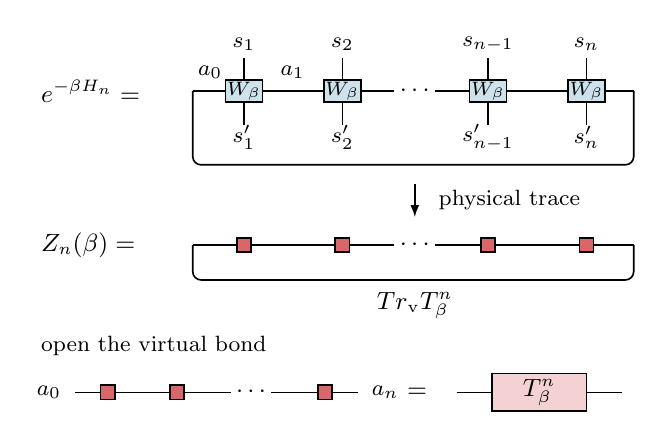
\begin{tikzpicture}[x=1cm,y=.85cm,font=\small]
 % A periodic MPO: virtual bonds close; physical input and output legs stay open.
 \node[anchor=west] at (.15,5.60) {$e^{-\beta H_n}=$};
 \draw[wire] (2.20,5.60)--(7.80,5.60);
 \draw[wire,rounded corners=3pt]
   (2.20,5.60)--(2.20,4.50)--(7.80,4.50)--(7.80,5.60);
 \foreach \x/\j in {2.85/1,4.10/2,5.95/{n-1},7.20/n}{
   \draw[wire] (\x,5.10)--(\x,6.10);
   \node[tensor,minimum width=.47cm,minimum height=.28cm,
     fill=mpoblue!30,font=\scriptsize] at (\x,5.60) {$W_\beta$};
   \node[font=\footnotesize] at (\x,6.30) {$s_{\j}$};
   \node[font=\footnotesize] at (\x,4.91) {$s'_{\j}$};}
 \node[fill=white,inner sep=2pt] at (5.02,5.60) {$\cdots$};
 \node[font=\footnotesize] at (2.42,5.88) {$a_0$};
 \node[font=\footnotesize] at (3.47,5.88) {$a_1$};
 \draw[arrow] (5.02,4.22)--(5.02,3.72);
 \node[anchor=west,font=\footnotesize] at (5.20,3.97) {physical trace};
 % Tracing every pair of physical legs leaves a periodic transfer chain.
 \node[anchor=west] at (.15,3.30) {$Z_n(\beta)=$};
 \draw[wire] (2.20,3.30)--(7.80,3.30);
 \draw[wire,rounded corners=3pt]
   (2.20,3.30)--(2.20,2.78)--(7.80,2.78)--(7.80,3.30);
 \foreach \x in {2.85,4.10,5.95,7.20}{
   \node[tensor,fill=mpored] at (\x,3.30) {};}
 \node[fill=white,inner sep=2pt] at (5.02,3.30) {$\cdots$};
 \node at (5.02,2.40) {$\trv\mathbb T_\beta^n$};
 % Cutting the closing virtual bond gives a transfer operator power.
 \node[anchor=west,font=\footnotesize] at (.15,1.80) {open the virtual bond};
 \draw[wire] (.70,1.10)--(4.30,1.10);
 \foreach \x in {1.12,2.00,3.88}{
   \node[tensor,fill=mpored] at (\x,1.10) {};}
 \node[fill=white,inner sep=2pt] at (2.94,1.10) {$\cdots$};
 \node[font=\footnotesize,anchor=east] at (.65,1.10) {$a_0$};
 \node[font=\footnotesize,anchor=west] at (4.35,1.10) {$a_n$};
 \node at (5.05,1.10) {$=$};
 \draw[wire] (5.55,1.10)--(7.65,1.10);
 \node[tensor,fill=mpored!30,minimum width=1.20cm,minimum height=.48cm]
   at (6.60,1.10) {$\mathbb T_\beta^n$};
\end{tikzpicture}
\end{proofdiagram}
The horizontal virtual bond closes with $a_n=a_0$; the vertical physical
legs $s_j,s'_j$ remain open. Tracing them gives the red ring. Cutting its
closing bond leaves $\mathbb T_\beta^n$; closing it takes the virtual
trace $\trv$.

This open chain defines a second normalized operator and purity:
\begin{equation}
 \begin{aligned}
 \sigma_n(\beta)&=\frac{\mathbb T_\beta^n}{Z_n(\beta)},\\
 \Ps(n,\beta)&=\trv\sigma_n(\beta)^2
 =\frac{Z_{2n}(\beta)}{Z_n(\beta)^2}.
 \end{aligned}
 \label{eq:spatialpurity}
\end{equation}
Because $n$ is even, $\sigma_n$ is positive with unit trace.
The transfer purity $\Ps$ compares lengths, while the Gibbs purity
$\Pt$ compares inverse temperatures.

\emph{The doubling estimate.---}
We will propagate the finite-size input using the following implication,
valid for $0\le\varepsilon\le1/100$:
\begin{equation}
 \begin{gathered}
 \Ps(n,\beta),\ \Pt(2n,\beta)\ge1-\varepsilon\\
 \Longrightarrow\quad
 \Ps(2n,2\beta),\ \Pt(4n,2\beta)\ge1-5\varepsilon^2.
 \end{gathered}
 \label{eq:update}
\end{equation}
This doubles both scales and replaces $\varepsilon$ by $5\varepsilon^2$.
To prove it, we
first bound the effect of squaring each operator, then relate the two
purities by joining copies of the MPO.

\emph{Proof of the doubling estimate.---}
Let $p_i$ and $w_m$ be the eigenvalues of $\sigma_n$ and $\rho_n$.
Squaring $\sigma_n$ doubles $n$; squaring $\rho_n$ doubles $\beta$:
\begin{proofdiagram}
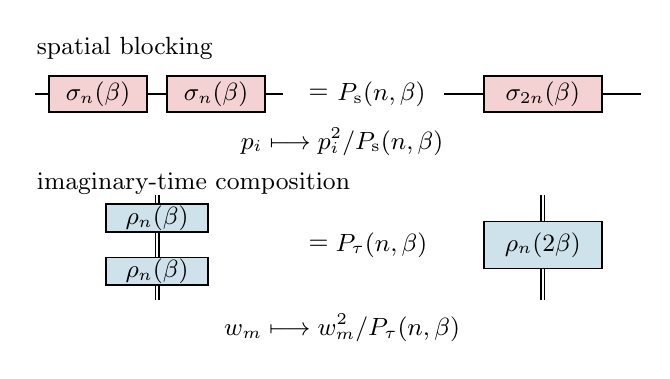
\begin{tikzpicture}[x=1cm,y=.90cm,font=\small]
 \node[anchor=west] at (0,2.00) {spatial blocking};
 \draw[wire] (.1,1.35)--(3.25,1.35);
 \node[tensor,fill=mpored!30,minimum width=1.25cm,minimum height=.45cm] at (.90,1.35) {$\sigma_n(\beta)$};
 \node[tensor,fill=mpored!30,minimum width=1.25cm,minimum height=.45cm] at (2.40,1.35) {$\sigma_n(\beta)$};
 \node at (3.70,1.35) {$=$};
 \node at (4.50,1.35) {$\Ps(n,\beta)$};
 \draw[wire] (5.30,1.35)--(7.80,1.35);
 \node[tensor,fill=mpored!30,minimum width=1.5cm,minimum height=.45cm] at (6.55,1.35) {$\sigma_{2n}(\beta)$};
 \node at (4,.68) {$p_i\longmapsto p_i^2/\Ps(n,\beta)$};
 \node[anchor=west] at (0,.08) {imaginary-time composition};
 \draw[wire,double distance=.6pt] (1.65,-.08)--(1.65,-1.55);
 \node[tensor,fill=mpoblue!30,minimum width=1.3cm,minimum height=.35cm] at (1.65,-.40) {$\rho_n(\beta)$};
 \node[tensor,fill=mpoblue!30,minimum width=1.3cm,minimum height=.35cm] at (1.65,-1.15) {$\rho_n(\beta)$};
 \node at (3.70,-.78) {$=$};
 \node at (4.50,-.78) {$\Pt(n,\beta)$};
 \draw[wire,double distance=.6pt] (6.55,-.08)--(6.55,-1.55);
 \node[tensor,fill=mpoblue!30,minimum width=1.5cm,minimum height=.6cm] at (6.55,-.78) {$\rho_n(2\beta)$};
 \node at (4,-1.95) {$w_m\longmapsto w_m^2/\Pt(n,\beta)$};
\end{tikzpicture}
\end{proofdiagram}
Double legs denote the $n$-site physical space. For either normalized
spectrum, write $P=\sum_i p_i^2$. After $p_i\mapsto p_i^2/P$, its new
purity $P'$ satisfies
\begin{equation}
 1-P'=\frac{2\sum_{i<k}p_i^2p_k^2}{P^2}
 \le\frac{(1-P)^2}{2P^2}=:f(1-P).
 \label{eq:square}
\end{equation}
Indeed, $1-P=2\sum_{i<k}p_ip_k$, and dropping cross terms from the square
of this sum gives the inequality. The function $f$ is increasing on
$[0,1)$ and behaves as $x^2/2$ for small $x$.

The squaring identities change one scale at a time. To double both, we need an
identity relating $\Ps$ and $\Pt$. Rejoin the trace loops of four copies
of $Z_n(\beta)$ in either order:
\begin{proofdiagram}
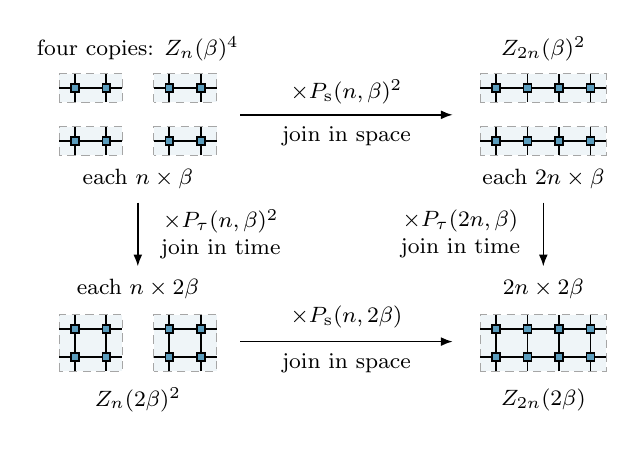
\begin{tikzpicture}[x=1cm,y=.90cm,font=\footnotesize]
 \netpatch{.35}{3.75}{2}{1}
 \netpatch{1.55}{3.75}{2}{1}
 \netpatch{.35}{4.50}{2}{1}
 \netpatch{1.55}{4.50}{2}{1}
 \node at (1.35,5.25) {four copies: $Z_n(\beta)^4$};
 \node at (1.35,3.42) {each $n\times\beta$};
 \netpatch{5.70}{3.75}{4}{1}
 \netpatch{5.70}{4.50}{4}{1}
 \node at (6.50,5.25) {$Z_{2n}(\beta)^2$};
 \node at (6.50,3.42) {each $2n\times\beta$};
 \draw[arrow] (2.65,4.32)--(5.35,4.32);
 \node at (4,4.64) {$\times \Ps(n,\beta)^2$};
 \node at (4,4.02) {join in space};
 \netpatch{.35}{.70}{2}{2}
 \netpatch{1.55}{.70}{2}{2}
 \node at (1.35,.30) {$Z_n(2\beta)^2$};
 \node at (1.35,1.86) {each $n\times2\beta$};
 \netpatch{5.70}{.70}{4}{2}
 \node at (6.50,.30) {$Z_{2n}(2\beta)$};
 \node at (6.50,1.86) {$2n\times2\beta$};
 \draw[arrow] (2.65,1.12)--(5.35,1.12);
 \node at (4,1.47) {$\times \Ps(n,2\beta)$};
 \node at (4,.81) {join in space};
 \draw[arrow] (1.35,3.08)--(1.35,2.18);
 \node[align=center,anchor=west] at (1.52,2.64)
   {$\times \Pt(n,\beta)^2$\\join in time};
 \draw[arrow] (6.50,3.08)--(6.50,2.18);
 \node[align=center,anchor=east] at (6.33,2.64)
   {$\times \Pt(2n,\beta)$\\join in time};
\end{tikzpicture}
\end{proofdiagram}
Each rectangle is periodic in both directions; its width and height
denote length and inverse temperature. Tensors are schematic, and
arrows give ratios of new to old contraction values. Both orders end
at $Z_{2n}(2\beta)$, so equating their ratios gives
\begin{align}
 \Ps(n,2\beta)&=\frac{\Ps(n,\beta)^2\Pt(2n,\beta)}{\Pt(n,\beta)^2},
 \label{eq:couple1}\\
 \Pt(4n,\beta)&=\frac{\Pt(2n,\beta)^2\Ps(2n,2\beta)}{\Ps(2n,\beta)^2}.
 \label{eq:couple2}
\end{align}
The second line is the same identity at length $2n$, solved for
$\Pt(4n,\beta)$. These identities explain the pair of lengths $n,2n$
in Eq.~\eqref{eq:update}.

Now assume $\Ps(n,\beta),\Pt(2n,\beta)\ge1-\varepsilon$.
Since all purities are at most one, Eq.~\eqref{eq:couple1} gives
$\Ps(n,2\beta)\ge(1-\varepsilon)^3$. Squaring the transfer operator
therefore gives $\Ps(2n,2\beta)\ge1-\delta$, where
\begin{equation}
 \delta=f\bigl(1-(1-\varepsilon)^3\bigr)
 =\tfrac12\bigl[(1-\varepsilon)^{-3}-1\bigr]^2
 \le5\varepsilon^2\le\varepsilon.
 \label{eq:delta}
\end{equation}
The bound uses $1-(1-\varepsilon)^3\le3\varepsilon$ and
$9/[2(1-3\varepsilon)^2]\le5$.

This proves the transfer-purity bound in Eq.~\eqref{eq:update}.
For the Gibbs-purity bound, insert it into Eq.~\eqref{eq:couple2}.
Using $\delta\le\varepsilon$ gives $\Pt(4n,\beta)\ge(1-\varepsilon)^3$.
Squaring the Gibbs operator then gives $\Pt(4n,2\beta)\ge1-\delta$.
Thus both bounds in Eq.~\eqref{eq:update} hold.

\emph{From finite input to all lengths.---}
We now apply the doubling estimate to Proposition~5.5 of
Ref.~\cite{source}:
\begin{equation}
 \Ps(2304,784),\ \Pt(4608,784)\ge0.99.
 \label{eq:input}
\end{equation}
The energy shift used there cancels from the purity ratios.
For $j\ge0$, set
\begin{equation}
 n_j=2304\,2^j,\qquad\beta_j=784\,2^j,\qquad
 \varepsilon_j=\frac{20^{-2^j}}5.
 \label{eq:scales}
\end{equation}
Since $\varepsilon_0=1/100$ and $\varepsilon_{j+1}=5\varepsilon_j^2$,
induction in Eq.~\eqref{eq:update} gives
$\Ps(n_j,\beta_j),\Pt(2n_j,\beta_j)\ge1-\varepsilon_j$.
The error bound is exponential in inverse temperature:
$\varepsilon_j=\frac15 e^{-\beta_j(\log20)/784}$.

To include every even $L\ge2304$, choose $j$ with $n_j\le L\le2n_j$.
The moment formula~\eqref{eq:moment} and monotonicity of $\ell^p$ norms give
\begin{align}
 Z_L(\beta_j)&\le Z_{n_j}(\beta_j)^{L/n_j},\notag\\
 Z_L(2\beta_j)&\ge Z_{2n_j}(2\beta_j)^{L/(2n_j)}.
 \label{eq:moments}
\end{align}
Substituting into the Gibbs-purity ratio~\eqref{eq:thermalpurity} yields
\begin{align}
 \Pt(L,\beta_j)
 &\ge\bigl[\Pt(2n_j,\beta_j)\Ps(n_j,\beta_j)^2\bigr]^{L/(2n_j)}\notag\\
 &\ge(1-\varepsilon_j)^3\ge1-3\varepsilon_j>\tfrac12.
 \label{eq:interpolate}
\end{align}
Here both purities in brackets are at least $1-\varepsilon_j$, and
$L/(2n_j)\le1$. This is the bound needed in Eq.~\eqref{eq:target}:
\begin{equation}
 e^{-\beta_j\Delta_L}
 \le\frac{3\varepsilon_j}{1-3\varepsilon_j}
 \le\frac{60}{97}\,20^{-2^j}<20^{-2^j}.
 \label{eq:gapratio}
\end{equation}
Taking logarithms and dividing by $\beta_j=784\,2^j$ proves
\begin{equation}
 \boxed{\Delta_L>\frac{\log20}{784}\simeq0.003821
 \quad(L\ge2304\text{ even}).}
 \label{eq:gap}
\end{equation}
Consequently, the ground state is unique for these lengths and
$\liminf_{L\to\infty,\;L\,\mathrm{even}}\Delta_L>0$.

\begin{acknowledgments}
We thank Shengqi Sang, Yimu Bao, and Xiao-Liang Qi for helpful discussions.
\end{acknowledgments}

\emph{AI-use declaration.---}
S.\,L. prompted GPT-6-Astra (OpenAI) to recast the proof of
Ref.~\cite{source} in tensor-network diagrams.

\begin{thebibliography}{3}
\bibitem{source}
OpenAI, \emph{The periodic spin-one Haldane gap}, manuscript dated
September 24, 2026, Proposition 5.5 and Appendices A--C.
\bibitem{tang}
W. Tang, H.-H. Tu, and L. Wang,
\href{https://doi.org/10.1103/PhysRevLett.125.170604}
{Continuous matrix product operator approach to finite temperature quantum states},
Phys. Rev. Lett. \textbf{125}, 170604 (2020).
\bibitem{pirvu}
B. Pirvu, V. Murg, J. I. Cirac, and F. Verstraete,
\href{https://doi.org/10.1088/1367-2630/12/2/025012}
{Matrix product operator representations},
New J. Phys. \textbf{12}, 025012 (2010).
\end{thebibliography}
\end{document}
